\label{forceana}
In setup 3 and setup 4, we stabilised each protein with an external force acting on the FERM domain (see \autoref{motivation}). To ensure that this restraining does not cause major artefacts, the force-dependency of the used observables is examined below.\\
\\
The force has a mean value of $2.44\,\forceunit$ and a standard deviation of $21.80\,\forceunit$. Interestingly, the positive mean value shows that the proteins are rather pushed downwards than pulled up. This indicates that the stabilising force does not have to hold the protein upright the whole time. % TODO: clarify?
\\
Linear regressions show that all of the quantities $d_\text{F}$ (distance between F1 and F2), $d_\text{F1-N}$, $d_\text{F2-C}$ and CA have a negligible correlation to the applied force. Here, negligible means that either the regression result was not significant or that the obtained slope was so small, that a change of one standard deviation in force would not change the quantity noticeably.\\
\\
We also tested the inter-residue distances for correlation with the applied force. To this end, 10 different proteins without neighbours were monitored, each for $1\,\si{\micro\second}$. For each residue pair in this dataset, we performed a linear regression. \autoref{force:contactmap} shows the calculated Pearson correlation coefficient (only significant correlations with Pearson $\left|r\right| > 0.3$). The mean value of the slope for the positively correlated pair distances is $33.7\,\si{\pico\newton/\nano\metre}$ and $-32.7\,\si{\pico\newton/\nano\metre}$ for the negatively correlated pair distances. Thus, the force can influence residue pairs contributing to the interface. However, we do not expect major changes in the contact regions, since the majority of residue pairs show only weak correlations.\\
%
%
%
\begin{figure}[h]
	\centering
	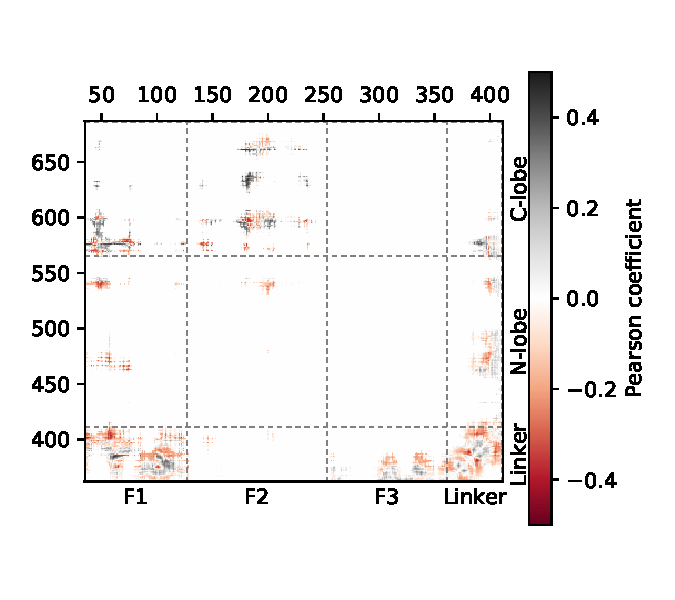
\includegraphics[width=.7\textwidth]{figures/results/interface_corr}
	\nicecaption{Correlations in contact map}{The contact map shows correlations between inter-residue distances and the stabilising force. The mean slope is $33.2\,\si{\pico\newton/\nano\metre}$, the maximal Pearson $r < 0.5$.}
	\label{force:contactmap}
\end{figure}
%
%
%
\\
In summary, we do not expect large perturbations of our observables due to the force. However, this approach has limitations. First, there could be binding poses in multiple FAK interactions requiring a large inclination of the FAK molecule. These states would be suppressed by the force. Another limitation is that the force does not only prevent tilts around the long axis of FAK (falling to sideways), but also around the short axis, which happens e.g. in FERM-FERM dimers. Lastly the reference to the z-axis is problematic. A reference to the membrane might be better, because it would involve membrane curvature as well.
